%%%%%%%%%%%%%%%%%%%%%%%%%%%%%%%%%%%%%%%%%%%%%%%%%%%%%%%%%%%%%%%%%%%%%%%%%%%%%%%
\documentclass[letterpaper,10pt,titlepage]{article}
%\usepackage[bitstream-charter]{mathdesign}
\usepackage{amsmath}
\usepackage{amsfonts}
\usepackage{amssymb}
\usepackage[ansinew]{inputenc}
\usepackage[OT1]{fontenc}
\usepackage{graphicx}
\usepackage{makeidx}
%
\makeindex{}
%%%%%%%%%%%%%%%%%%%%%%%%%%%%%%%%%%%%%%%%%%%%%%%%%%%%%%%%%%%%%%%%%%%%%%%%%%%%%%%
\begin{document}
\title{Practices to Prevent Intermittent Software Defects in Software Targeted for 
       NXP\textsuperscript{\textregistered}
       Power Architecture\textsuperscript{\textregistered} Single-Core and 
	   Multi-Core Microcontrollers
	   with Green Hills Software\textsuperscript{\textregistered} C/C++ Compilers
	   under Vector\textsuperscript{\textregistered}
	   MICROSAR\textsuperscript{\textregistered}}
\author{\vspace{3cm}\\David T. Ashley\\\texttt{dashley@gmail.com}\\\vspace{3cm}}
\date{\LaTeX{} Compilation Date: \today{}}
\maketitle
%
%%%%%%%%%%%%%%%%%%%%%%%%%%%%%%%%%%%%%%%%%%%%%%%%%%%%%%%%%%%%%%%%%%%%%%%%%%%%%%%
%
\begin{abstract}
This document describes common causes of intermittent software defects
in embedded software (some of which are generic to all microcontroller
software, and some of which require specific hardware features).  Technical
background about these causes is also provided.

Information about architectural features of the 
Power Architecture\textsuperscript{\textregistered} family of processors is
provided, especially as it relates to intermittent software defects and how
to avoid producing software containing these intermittent software defects.

Information about NXP\textsuperscript{\textregistered} single-core and
multi-core microcontrollers that incorporate
Power Architecture\textsuperscript{\textregistered} processor cores is provided,
especially as it relates to intermittent software defects and how to avoid
producing software containing these intermittent defects.

Information about C/C++ compilers and the 
Green Hills Software\textsuperscript{\textregistered} C/C++ compilers
is provided,
especially as it relates to intermittent software defects and how to avoid
producing software containing these intermittent defects.
\end{abstract}

%%%%%%%%%%%%%%%%%%%%%%%%%%%%%%%%%%%%%%%%%%%%%%%%%%%%%%%%%%%%%%%%%%%%%%%%%%%%%%%
\pagenumbering{roman}
\tableofcontents{}
\clearpage{}
\listoffigures{}
\listoftables{}
\clearpage{}
\pagenumbering{arabic}
%%%%%%%%%%%%%%%%%%%%%%%%%%%%%%%%%%%%%%%%%%%%%%%%%%%%%%%%%%%%%%%%%%%%%%%%%%%%%%%

%Introduction and Overview
%%%%%%%%%%%%%%%%%%%%%%%%%%%%%%%%%%%%%%%%%%%%%%%%%%%%%%%%%%%%%%%%%%%%%%%%%%%%%%%
\section{Introduction and Overview}
\label{siov0}

\index{TBD}TBD.


%%%%%%%%%%%%%%%%%%%%%%%%%%%%%%%%%%%%%%%%%%%%%%%%%%%%%%%%%%%%%%%%%%%%%%%%%%%%%%%
\subsection{Scope and Purpose}
\label{siov0:sspu0}

TBD.


%%%%%%%%%%%%%%%%%%%%%%%%%%%%%%%%%%%%%%%%%%%%%%%%%%%%%%%%%%%%%%%%%%%%%%%%%%%%%%%
\subsection{Acknowledgments}
\label{siov0:sack0}

TBD.


%%%%%%%%%%%%%%%%%%%%%%%%%%%%%%%%%%%%%%%%%%%%%%%%%%%%%%%%%%%%%%%%%%%%%%%%%%%%%%%
\subsection{Trademarks and Service Marks}
\label{siov0:stsm0}

TBD.


%%%%%%%%%%%%%%%%%%%%%%%%%%%%%%%%%%%%%%%%%%%%%%%%%%%%%%%%%%%%%%%%%%%%%%%%%%%%%%%
\subsection{Permission to Include Copyrighted Material}
\label{siov0:spcr0}

TBD.


%%%%%%%%%%%%%%%%%%%%%%%%%%%%%%%%%%%%%%%%%%%%%%%%%%%%%%%%%%%%%%%%%%%%%%%%%%%%%%%
\subsection{License}
\label{siov0:slic0}

TBD.


\begin{figure}
\centering
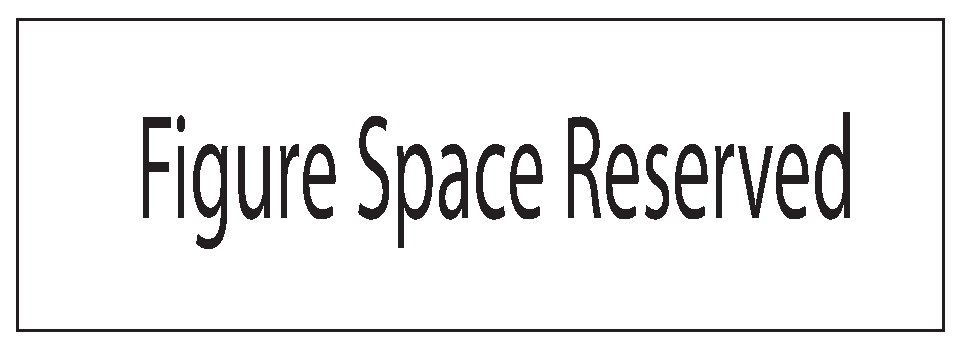
\includegraphics[width=4.6in]{common/figure_reserved.eps}
\caption{Reserved Figure}
\label{fig:siov0:01}
\end{figure}

\begin{table}
\caption{Reserved Table}
\label{tbl:siov0:01}
\begin{center}
\begin{tabular}{|c|c|c|c|c|}
\hline
\small{Index} & \small{$dividend_k$}  & \small{$divisor_k$} & \small{$a_k$}   & \small{$remainder_k$} \\
\small{($k$)} &                       &                     &                 &                       \\
\hline
\hline
\small{-1}    & \small{N/A}           & \small{67}          & \small{N/A}     & \small{29}            \\
\hline
\small{0}     & \small{67}            & \small{29}          & \small{2}       & \small{9}             \\
\hline
\small{1}     & \small{29}            & \small{9}           & \small{3}       & \small{2}             \\
\hline
\small{2}     & \small{9}             & \small{2}           & \small{4}       & \small{1}             \\
\hline
\small{3}     & \small{2}             & \small{1}           & \small{2}       & \small{0}             \\
\hline
\end{tabular}
\end{center}
\end{table}



%Common Features of Processors and Microcontrollers
%%%%%%%%%%%%%%%%%%%%%%%%%%%%%%%%%%%%%%%%%%%%%%%%%%%%%%%%%%%%%%%%%%%%%%%%%%%%%%%
\section{Common Features of Processors and Microcontrollers}
\label{scfp0}

TBD.


%%%%%%%%%%%%%%%%%%%%%%%%%%%%%%%%%%%%%%%%%%%%%%%%%%%%%%%%%%%%%%%%%%%%%%%%%%%%%%%
\subsection{FLASH Memory and FLASH Memory Restrictions}
\label{scfp0:sfmr0}

TBD.


%%%%%%%%%%%%%%%%%%%%%%%%%%%%%%%%%%%%%%%%%%%%%%%%%%%%%%%%%%%%%%%%%%%%%%%%%%%%%%%
\subsection{Instruction Cache}
\label{scfp0:sica0}

TBD.


%%%%%%%%%%%%%%%%%%%%%%%%%%%%%%%%%%%%%%%%%%%%%%%%%%%%%%%%%%%%%%%%%%%%%%%%%%%%%%%
\subsection{Data Cache}
\label{scfp0:sdca0}

TBD.


%%%%%%%%%%%%%%%%%%%%%%%%%%%%%%%%%%%%%%%%%%%%%%%%%%%%%%%%%%%%%%%%%%%%%%%%%%%%%%%
\subsection{Multi-Core Architectures}
\label{scfp0:smca0}

TBD.


%%%%%%%%%%%%%%%%%%%%%%%%%%%%%%%%%%%%%%%%%%%%%%%%%%%%%%%%%%%%%%%%%%%%%%%%%%%%%%%
\subsection{Multi-Core Cache and Cache Coherency Model}
\label{scfp0:smcc0}

TBD.


%%%%%%%%%%%%%%%%%%%%%%%%%%%%%%%%%%%%%%%%%%%%%%%%%%%%%%%%%%%%%%%%%%%%%%%%%%%%%%%
\subsection{Instruction Pipeline}
\label{scfp0:spip0}

TBD.


%%%%%%%%%%%%%%%%%%%%%%%%%%%%%%%%%%%%%%%%%%%%%%%%%%%%%%%%%%%%%%%%%%%%%%%%%%%%%%%
\subsection{Out-of-Order Memory Accesses}
\label{scfp0:soom0}

TBD.


%%%%%%%%%%%%%%%%%%%%%%%%%%%%%%%%%%%%%%%%%%%%%%%%%%%%%%%%%%%%%%%%%%%%%%%%%%%%%%%
\subsection{Memory Barrier Instructions}
\label{scfp0:smbi0}

TBD.


%%%%%%%%%%%%%%%%%%%%%%%%%%%%%%%%%%%%%%%%%%%%%%%%%%%%%%%%%%%%%%%%%%%%%%%%%%%%%%%
\subsection{Branch Prediction}
\label{scfp0:sbpd0}

TBD.


%%%%%%%%%%%%%%%%%%%%%%%%%%%%%%%%%%%%%%%%%%%%%%%%%%%%%%%%%%%%%%%%%%%%%%%%%%%%%%%
\subsection{Speculative Execution and Speculative Memory Accesses}
\label{scfp0:sses0}

TBD.


%%%%%%%%%%%%%%%%%%%%%%%%%%%%%%%%%%%%%%%%%%%%%%%%%%%%%%%%%%%%%%%%%%%%%%%%%%%%%%%
\subsection{Interrupts}
\label{scfp0:sint0}

TBD.


%%%%%%%%%%%%%%%%%%%%%%%%%%%%%%%%%%%%%%%%%%%%%%%%%%%%%%%%%%%%%%%%%%%%%%%%%%%%%%%
\subsubsection{General Description}
\label{scfp0:sint0:sovr0}

TBD.


%%%%%%%%%%%%%%%%%%%%%%%%%%%%%%%%%%%%%%%%%%%%%%%%%%%%%%%%%%%%%%%%%%%%%%%%%%%%%%%
\subsubsection{Atomic vs. Non-Atomic ISRs}
\label{scfp0:sint0:sana0}

TBD.


%%%%%%%%%%%%%%%%%%%%%%%%%%%%%%%%%%%%%%%%%%%%%%%%%%%%%%%%%%%%%%%%%%%%%%%%%%%%%%%
\subsubsection{Ability to Disable and Enable All Interrupts}
\label{scfp0:sint0:sdii0}

TBD.


%%%%%%%%%%%%%%%%%%%%%%%%%%%%%%%%%%%%%%%%%%%%%%%%%%%%%%%%%%%%%%%%%%%%%%%%%%%%%%%
\subsubsection{Ability to Disable and Enable Specific Interrupt Sources}
\label{scfp0:sint0:sdis0}

TBD.


%%%%%%%%%%%%%%%%%%%%%%%%%%%%%%%%%%%%%%%%%%%%%%%%%%%%%%%%%%%%%%%%%%%%%%%%%%%%%%%
\subsubsection{Use of Alternate Stack Pointer}
\label{scfp0:sint0:suas0}

TBD.


%%%%%%%%%%%%%%%%%%%%%%%%%%%%%%%%%%%%%%%%%%%%%%%%%%%%%%%%%%%%%%%%%%%%%%%%%%%%%%%
\subsection{TSL (Test-and-Set-Lock) and Similar Instructions}
\label{scfp0:stsl0}

TBD.



%%%%%%%%%%%%%%%%%%%%%%%%%%%%%%%%%%%%%%%%%%%%%%%%%%%%%%%%%%%%%%%%%%%%%%%%%%%%%%%
\subsection{Hardware Support for Concurrent Programming}
\label{scfp0:shsc0}

TBD.


%Features of the Power Architecture Family of Processors
%%%%%%%%%%%%%%%%%%%%%%%%%%%%%%%%%%%%%%%%%%%%%%%%%%%%%%%%%%%%%%%%%%%%%%%%%%%%%%%
\section{Features of the Power Architecture\textsuperscript{\textregistered}
         Family of Processors}
\label{sfpa0}

TBD.


%%%%%%%%%%%%%%%%%%%%%%%%%%%%%%%%%%%%%%%%%%%%%%%%%%%%%%%%%%%%%%%%%%%%%%%%%%%%%%%
\subsection{History and Defining Documents}
\label{sfpa0:shdd0}

TBD.


%%%%%%%%%%%%%%%%%%%%%%%%%%%%%%%%%%%%%%%%%%%%%%%%%%%%%%%%%%%%%%%%%%%%%%%%%%%%%%%
\subsection{Memory Model}
\label{sfpa0:smmo0}

TBD.



%Features of NXP Single-Core and Multi-Core Microcontrollers that Incorporate
%Power Architecture Processor Cores
%%%%%%%%%%%%%%%%%%%%%%%%%%%%%%%%%%%%%%%%%%%%%%%%%%%%%%%%%%%%%%%%%%%%%%%%%%%%%%%
\section{Features of NXP\textsuperscript{\textregistered} Single-Core and
         Multi-Core Microcontrollers that Incorporate
         Power Architecture\textsuperscript{\textregistered} Processor Cores}
\label{sndv0}

TBD.


%%%%%%%%%%%%%%%%%%%%%%%%%%%%%%%%%%%%%%%%%%%%%%%%%%%%%%%%%%%%%%%%%%%%%%%%%%%%%%%
\subsection{Defining Documents}
\label{sndv0:sddo0}

TBD.


%%%%%%%%%%%%%%%%%%%%%%%%%%%%%%%%%%%%%%%%%%%%%%%%%%%%%%%%%%%%%%%%%%%%%%%%%%%%%%%
\subsection{FLASH Memory Banks}
\label{sndv0:sfmb0}

TBD.


%%%%%%%%%%%%%%%%%%%%%%%%%%%%%%%%%%%%%%%%%%%%%%%%%%%%%%%%%%%%%%%%%%%%%%%%%%%%%%%
\subsection{Cache Coherency Model}
\label{sndv0:sccm0}

TBD.


%Features of the C/C++ Programming Language and Practical Compilers
%%%%%%%%%%%%%%%%%%%%%%%%%%%%%%%%%%%%%%%%%%%%%%%%%%%%%%%%%%%%%%%%%%%%%%%%%%%%%%%
\section{Features of the C/C++ Programming Language and Practical Compilers}
\label{scco0}

TBD.


%Features of the Green Hills Software C/C++ Compilers
%%%%%%%%%%%%%%%%%%%%%%%%%%%%%%%%%%%%%%%%%%%%%%%%%%%%%%%%%%%%%%%%%%%%%%%%%%%%%%%
\section{Features of the Green Hills Software\textsuperscript{\textregistered}
         C/C++ Compilers}
\label{sghc0}

TBD.


%%%%%%%%%%%%%%%%%%%%%%%%%%%%%%%%%%%%%%%%%%%%%%%%%%%%%%%%%%%%%%%%%%%%%%%%%%%%%%%
\subsection{Compiler Barriers}
\label{sghc0:scba0}

TBD.


%%%%%%%%%%%%%%%%%%%%%%%%%%%%%%%%%%%%%%%%%%%%%%%%%%%%%%%%%%%%%%%%%%%%%%%%%%%%%%%
\subsection{Intrinsic Functions to Insert Memory Barrier Instructions}
\label{sghc0:sifu0}

TBD.


%Algorithms and Techniques for Concurrent Programming
%%%%%%%%%%%%%%%%%%%%%%%%%%%%%%%%%%%%%%%%%%%%%%%%%%%%%%%%%%%%%%%%%%%%%%%%%%%%%%%
\section{Algorithms and Techniques for Concurrent Programming}
\label{satq0}

TBD.


%%%%%%%%%%%%%%%%%%%%%%%%%%%%%%%%%%%%%%%%%%%%%%%%%%%%%%%%%%%%%%%%%%%%%%%%%%%%%%%
\subsection{Locking Algorithms and Techniques}
\label{satq0:sloc0}

TBD.


%%%%%%%%%%%%%%%%%%%%%%%%%%%%%%%%%%%%%%%%%%%%%%%%%%%%%%%%%%%%%%%%%%%%%%%%%%%%%%%
\subsection{Non-Locking Algorithms and Techniques}
\label{satq0:snlo0}

TBD.


%Implementation of Concurrent Programming Techniques on NXP Single-Core and
%Multi-Core Microcontrollers that Incorporate Power Architecture Processor
%Cores
%%%%%%%%%%%%%%%%%%%%%%%%%%%%%%%%%%%%%%%%%%%%%%%%%%%%%%%%%%%%%%%%%%%%%%%%%%%%%%%
\section{Implementation of Concurrent Programming Techniques on
         NXP\textsuperscript{\textregistered} Single-Core and
         Multi-Core Microcontrollers that Incorporate
         Power Architecture\textsuperscript{\textregistered} Processor Cores}
\label{sicp0}

TBD.



%Common Software Design Patterns
%%%%%%%%%%%%%%%%%%%%%%%%%%%%%%%%%%%%%%%%%%%%%%%%%%%%%%%%%%%%%%%%%%%%%%%%%%%%%%%
\section{Common Software Design Patterns}
\label{scsd0}

TBD.


%Common Causes and Mechanisms of Intermittent Software Defects
%%%%%%%%%%%%%%%%%%%%%%%%%%%%%%%%%%%%%%%%%%%%%%%%%%%%%%%%%%%%%%%%%%%%%%%%%%%%%%%
\section{Common Causes and Mechanisms of Intermittent Software Defects}
\label{scmd0}

Would like to cite one author \cite{lamport94}, then another author \cite{lamport95}.
Would also like to cite portions of a work, such as \cite[p. 314]{lamport95}


%%%%%%%%%%%%%%%%%%%%%%%%%%%%%%%%%%%%%%%%%%%%%%%%%%%%%%%%%%%%%%%%%%%%%%%%%%%%%%%
\subsection{Failure to Write RAM Before Reading}
\label{scmd0:sfwr0}

TBD.


%%%%%%%%%%%%%%%%%%%%%%%%%%%%%%%%%%%%%%%%%%%%%%%%%%%%%%%%%%%%%%%%%%%%%%%%%%%%%%%
\subsection{Failure to Provide Mutual Exclusion}
\label{scmd0:sfme0}

TBD.


%%%%%%%%%%%%%%%%%%%%%%%%%%%%%%%%%%%%%%%%%%%%%%%%%%%%%%%%%%%%%%%%%%%%%%%%%%%%%%%
\subsubsection{Incorrect Operations on Machine Control Registers}
\label{scmd0:siom0}

TBD.



%%%%%%%%%%%%%%%%%%%%%%%%%%%%%%%%%%%%%%%%%%%%%%%%%%%%%%%%%%%%%%%%%%%%%%%%%%%%%%%
\subsubsection{Incorrect Assumption About Atomicity of C Statement}
\label{scmd0:siac0}

TBD.


%%%%%%%%%%%%%%%%%%%%%%%%%%%%%%%%%%%%%%%%%%%%%%%%%%%%%%%%%%%%%%%%%%%%%%%%%%%%%%%
\subsection{Allowing an ISR to Run Too Early in the Initialization
            of the Software}
\label{scmd0:sait0}

TBD.


%%%%%%%%%%%%%%%%%%%%%%%%%%%%%%%%%%%%%%%%%%%%%%%%%%%%%%%%%%%%%%%%%%%%%%%%%%%%%%%
\subsection{Failure to Run ISR Within a Deadline}
\label{scmd0:sfid0}

TBD.



%Best Practices for the Prevention of Intermittent Software Defects
%%%%%%%%%%%%%%%%%%%%%%%%%%%%%%%%%%%%%%%%%%%%%%%%%%%%%%%%%%%%%%%%%%%%%%%%%%%%%%%
\section{Best Practices for the Prevention of Intermittent Software Defects}
\label{sbpp0}

TBD.


%References
%%%%%%%%%%%%%%%%%%%%%%%%%%%%%%%%%%%%%%%%%%%%%%%%%%%%%%%%%%%%%%%%%%%%%%%%%%%%%%%
\clearpage
\addcontentsline{toc}{section}{References}

\begin{thebibliography}{999}

\bibitem{lamport94}
  Leslie Lamport,
  \emph{\LaTeX: A Document Preparation System}.
  Addison Wesley, Massachusetts,
  2nd Edition,
  1994.

\bibitem{lamport95}
  John Smith
  \emph{\LaTeX: A Second Book}.
  Addison Wesley, Massachusetts,
  2nd Edition,
  1994.

\end{thebibliography}

%Index
%%%%%%%%%%%%%%%%%%%%%%%%%%%%%%%%%%%%%%%%%%%%%%%%%%%%%%%%%%%%%%%%%%%%%%%%%%%%%%%
\clearpage
\addcontentsline{toc}{section}{Index}
\printindex{}


%%%%%%%%%%%%%%%%%%%%%%%%%%%%%%%%%%%%%%%%%%%%%%%%%%%%%%%%%%%%%%%%%%%%%%%%%%%%%%%
\end{document}
%%%%%%%%%%%%%%%%%%%%%%%%%%%%%%%%%%%%%%%%%%%%%%%%%%%%%%%%%%%%%%%%%%%%%%%%%%%%%%%
